% =============================================================================
% CAPÍTULO 3 — a raiz (AGENTS.md §6): a medida, o corte e o preço de fixar.
%
% O fracasso que o abre, com número na mão: a linha erguida no décimo terceiro pior
% dia dos últimos 252 pregões entrega 5,135% contra os 5% anunciados — parece
% cumprida —, mas o pior bloco de 60 dias tem 20 violações onde a promessa admitia
% 3, e nenhum dos 200 mundos que nunca mudam passou de 13.
%
% Medição: lab/experimentos/E01_promessa.ipynb. Figuras: figuras/E01_promessa_*.
% =============================================================================

\chapter{A medida, o corte e o preço}
\label{cap:medida}

\section{Quanto eu posso perder amanhã}

O mercado fecha, e a pergunta volta quase toda noite com as mesmas palavras: quanto eu posso
perder amanhã? Quem carrega dinheiro aplicado não pergunta por gosto de adivinhar, porque a
resposta decide se a posição cabe no bolso de quem a carrega; e a posição que não cabe acaba
desmontada, muitas vezes antes de o mercado explicar o que estava acontecendo.

Responder exige duas decisões, e as duas são sobre o passado. A primeira é quantos dias olhar
para trás. A segunda é onde pôr a linha dentro desses dias, que podem ser o pior de todos, o
segundo pior, o décimo terceiro. Escrita por inteiro, a regra soa assim: \emph{o corte de hoje
é o décimo terceiro pior dia dos últimos \numCorteJanela{} pregões}. Ela também traz o que
pretende valer: \emph{não passo daqui, dezenove dias em vinte}, que é o mesmo que prometer
\numPromessaPct\% de violação.

Vale fixar quatro palavras, porque nenhuma delas muda de sentido daqui em diante: a
\textbf{janela} é o pedaço do passado que a regra olha; o \textbf{corte} é onde a linha é posta
dentro da janela; a \textbf{promessa} é a taxa de violação que se anuncia; e a \textbf{entrega}
é a taxa que de fato acontece.

A linha posta no quantil dos piores dias sustenta a medida de risco mais usada em finanças,
discutida e corrigida há décadas \cite{oconnell2026extreme}.
% aterramento: quantil
O quantil de uma fração declarada é o valor que deixa essa fração dos dias abaixo dele, e é ele
que o corte usa aqui. Com cem dias e a fração de um quinto, o quantil é o vigésimo pior dia:
vinte dos cem ficam abaixo dele. O que se pergunta vem antes disso, e é bem menor: a entrega tem
alguma coisa a ver com a promessa?

\section{O dado e a regra}

O dado é o retorno de um dia para o outro, que o capítulo anterior escreveu como o logaritmo
da razão entre dois preços:

\[
  r_{t+1} = \log \frac{p_{t+1}}{p_t}.
\]

O retorno é o incremento e o preço é o nível: empilhar dias é somar retornos, e é isso que
permite acompanhar o dia a dia sem perder o fio da conta.

A série é o índice S\&P 500, % numeros-ok: nome próprio, não medição
com \numSerieDias{} pregões, de \numSerieInicio{} a \numSerieFim. Ela vem do arquivo do
projeto anterior, e o empréstimo fica declarado: o dado atravessa, e todo número tirado dele é
medido de novo aqui.

Sobre essa série a regra toma duas decisões, e só duas. A \textbf{janela}: os
\numCorteJanela{} pregões anteriores a hoje. O \textbf{corte}: o décimo terceiro pior deles.
O corte de cada dia é erguido com os dias que já passaram e com nenhum outro, de modo que a
linha que aparece no gráfico estava lá antes de o dia acontecer. Um corte que espiasse o
futuro acertaria sempre, e por isso não valeria nada.

\section{A conta que o corte faz sozinho}

Nos \numEntregaDias{} dias em que havia janela suficiente, a linha foi rompida
\numEntregaViolacoes{} vezes. Isso dá \numEntregaTaxaPct\% de entrega, contra os
\numPromessaPct\% anunciados, uma diferença de pouco mais de um décimo de ponto percentual, pequena o
bastante para deixar a impressão de que a regra funcionou.

A impressão engana, e o motivo é aritmético. Quem decidiu o número foi o gesto de erguer a
linha dentro da janela, e não o que o mercado fez depois.

% aterramento: k
% aterramento: n
Vale dar nome às duas peças da decisão, porque a conta inteira se escreve com elas: $n$ é o
número de dias da janela, e $k$ é o posto do corte dentro dela --- o lugar que a linha ocupa na
fila dos piores dias. O corte é o décimo terceiro pior, de modo que aqui $k$ é treze e $n$ é
\numCorteJanela.

\begin{proposicao}[a conta do corte]
\label{prop:conta}
Suponha que os $n$ dias da janela e o dia seguinte sejam $n+1$ valores de uma mesma lei
contínua, em qualquer ordem igualmente provável. Se o corte é o $k$-ésimo menor dos $n$
dias da janela, então a probabilidade de o dia seguinte ficar abaixo do corte é
$\dfrac{k}{n+1}$.
\end{proposicao}

\begin{proof}
Junte os $n+1$ valores e ponha-os em ordem crescente. Todas as ordens são igualmente
prováveis, então a posição do dia seguinte nessa fila é uniforme entre as $n+1$ posições. O
dia seguinte fica abaixo do corte exatamente quando ocupa uma das $k$ primeiras posições da
fila dos $n+1$ valores. Logo a probabilidade é $k/(n+1)$.
\end{proof}

A lei ser contínua serve para que dias empatados tenham probabilidade zero; e a hipótese de
que todas as ordens são igualmente prováveis é a hipótese de que os dias não têm nada a dizer
uns sobre os outros, que é justamente o que um mundo que muda viola\cite{vovk2022algorithmic}. A proposição não prevê o
que vai acontecer. Ela é o contraste contra o qual o que aconteceu se lê.

Ela também é um caso pequeno e exato de um viés conhecido. Uma \textbf{amostra} é o pedaço
finito de dias de que se dispõe --- aqui, a janela ---, e um \textbf{viés} é o erro que a própria
regra assina antes de o dado chegar, e que por isso não vem do mundo.
% aterramento: amostra
% aterramento: vies
O quantil estimado de uma amostra não entrega a probabilidade que se anuncia, e o tamanho do
erro depende do tamanho da amostra \cite{taleb2020super}.

Com $n = \numCorteJanela$ e $k = \numCortePosto$, a conta dá
$\numCortePosto/(\numCorteJanela+1)$, que é \numCorteContaPct\%. Esse número não veio do
mercado, e sim da decisão de olhar \numCorteJanela{} dias e cortar no décimo terceiro. Se o
posto fosse o décimo segundo, a conta daria \numCorteAlternativoPct\%; e a promessa anunciada
não está em nenhum dos dois, porque o posto teria de cair entre o décimo segundo e o décimo
terceiro, e posto fracionário não existe.

O mercado entregou \numEntregaTaxaPct\%: \numEntregaViolacoes{} rompimentos em
\numEntregaDias{} dias, com poucos milésimos de diferença da conta do corte. Para saber se
essa diferença diz alguma coisa, falta o contraste que responde, e ele pede um mundo em que
nada muda submetido à mesma rotina.
% aterramento: mundo-parado
A esse contraste dou um nome, porque ele volta quase toda vez daqui em diante: o \textbf{mundo
que nunca muda}.

Sorteamos \numNuncaMudaMundos{} séries do tamanho da nossa, com retornos independentes e
sempre a mesma lei, e aplicamos a cada uma a mesma regra. A entrega média desses mundos foi
\numNuncaMudaTaxaPct\%, contra os \numCorteContaPct\% da conta; o mundo real entregou
\numEntregaTaxaPct\%. Os três números estão no mesmo lugar.

A média de violações é uma propriedade do corte, e não do mundo. O corte assinou o número
antes de qualquer dado chegar, e quem lê só a média lê a própria escolha acreditando estar
lendo o mercado.

\section{Os blocos têm data}

A diferença entre os mundos aparece na \emph{forma} com que as violações chegam: espalhadas
pelo calendário, ou concentradas em pedaços. Para medir a forma, contamos quantas violações
caem em cada janela móvel de \numBlocoDias{} dias --- a isso chamamos um \textbf{bloco} ---
e olhamos o bloco mais cheio. A promessa de \numPromessaPct\% admite \numBlocoPrometido{}
violações em \numBlocoDias{} dias.

% aterramento: mediana
A mediana dos blocos é \numBlocoMediana. A mediana é o quantil de metade: metade dos blocos tem
menos violações que ela, e a outra metade tem mais. Na maior parte do tempo a linha aguenta mais
do que prometeu. O pior bloco tem \numBlocoPior{} violações, e termina em \numBlocoPiorData. Onde a
promessa admitia \numBlocoPrometido{}, aconteceram \numBlocoPior.

Nos \numNuncaMudaMundos{} mundos que nunca mudam, o pior bloco de cada um teve, em média,
\numNuncaMudaPiorMedio{} violações, e o pior bloco de todos eles chegou a
\numNuncaMudaPiorBloco. Nenhum passou disso. A série real, com o mesmo tamanho e a mesma
rotina, chegou a \numBlocoPior.

\begin{figure}[htbp]
  \centering
  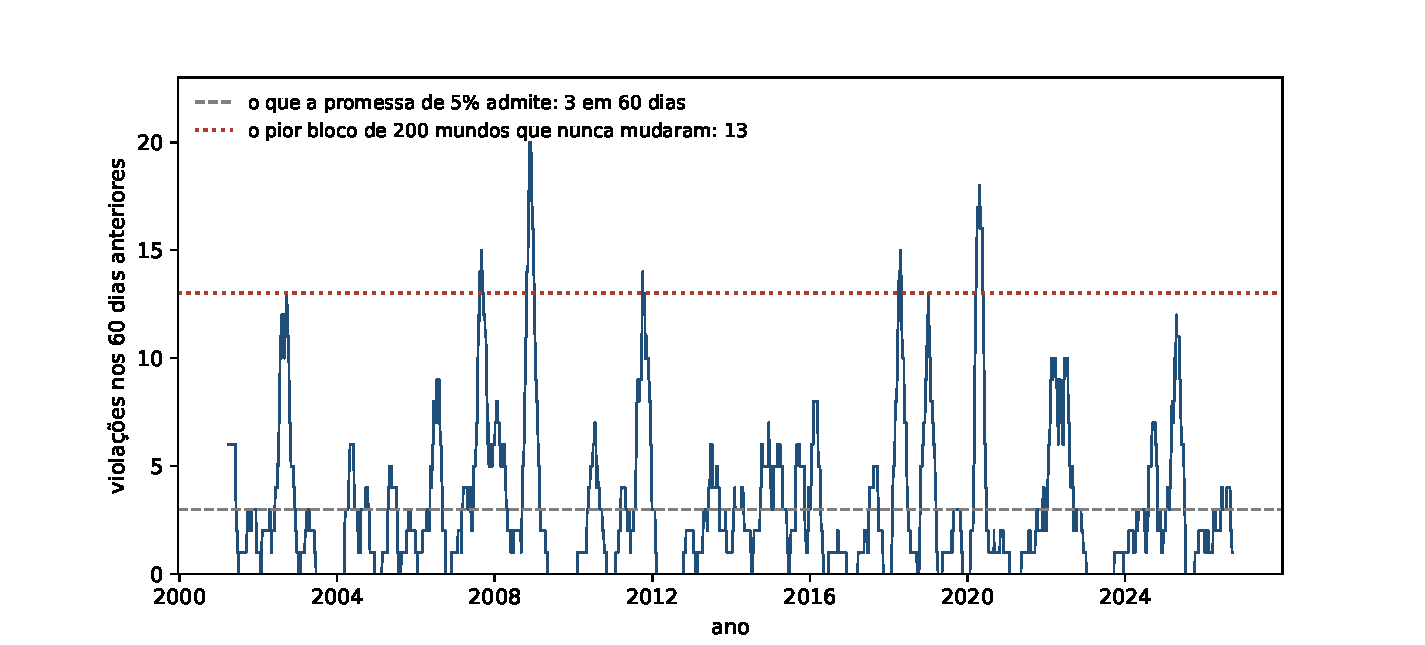
\includegraphics[width=\linewidth]{figuras/E01_promessa_1.pdf}
  \caption{Violações nos \numBlocoDias{} dias anteriores, dia a dia. A linha tracejada marca o
    que a promessa de \numPromessaPct\% admite; a pontilhada marca o pior bloco que apareceu
    em \numNuncaMudaMundos{} mundos que nunca mudam.}
  \label{fig:blocos}
\end{figure}

A escala do desenho trabalha contra a leitura. A linha da promessa fica rente ao chão do quadro, e é
ali que a série passa a maior parte do tempo; um eixo cortado perto dela devolveria um desenho de
promessa cumprida, e os surtos que cruzam o teto desapareceriam por recorte.

A figura mostra o que a média esconde. A série passa trechos longos colada na linha da
promessa e sobe, em surtos curtos, até cruzar a linha pontilhada. E os blocos têm data: o teto
dos mundos que nunca mudam é cruzado em \numEpisodiosAcimaDoTeto{} episódios distintos, dois deles em dois mil e
sete, que ocupam \numBlocosAcimaDoTetoPct\% dos blocos medidos, em \numEpisodiosAnos. Nem todos esses
anos têm nome de crise, e todos aconteceram neste mercado.

A leitura do bloco corrige ainda a primeira impressão: \numBlocoAcimaDoDobroPct\% dos blocos
passam do dobro da promessa. O que se promete fica longe do que se entrega, tanto na maior
parte do tempo quanto nos piores pedaços, e a entrega acaba sendo uma média entre os dois.

\section{O preço muda de lugar}

Se o corte assina a média, uma saída parece evidente: escolher outra janela. Vale a pena
tentar, e a tentativa é barata, porque é a mesma regra com outro número. Varremos a janela de
um mês a cinco anos, mantendo a promessa anunciada de \numPromessaPct\% e o bloco de
\numBlocoDias{} dias.

\begin{table}[htbp]
  \centering
  \begin{tabular}{rrrr}
    \hline
    janela & a conta do corte & a entrega & o pior bloco \\
    (pregões) & (\%) & (\%) & (violações) \\
    \hline
    \numCorteCurtoJanela & \numCorteCurtoContaPct & \numCorteCurtoTaxaPct & \numCorteCurtoPiorBloco \\
    \numCorteMedioJanela & \numCorteMedioContaPct & \numCorteMedioTaxaPct & \numCorteMedioPiorBloco \\
    \numCorteJanela & \numCorteContaPct & \numEntregaTaxaPct & \numBlocoPior \\
    \numCorteLongoJanela & \numCorteLongoContaPct & \numCorteLongoTaxaPct & \numCorteLongoPiorBloco \\
    \hline
  \end{tabular}
  \caption{A mesma regra com quatro janelas, a mesma promessa anunciada de
    \numPromessaPct\% e o mesmo bloco de \numBlocoDias{} dias. A coluna do meio segue a
    \cref{prop:conta}; a última traz o pior bloco medido.}
  \label{tab:varredura}
\end{table}

As três colunas respondem à pergunta do começo.

A \textbf{conta do corte} obedece à promessa anunciada apenas na janela longa. Na janela de um
mês, o corte assina \numCorteCurtoContaPct\%, quase o dobro dos \numPromessaPct\% anunciados,
e a razão disso é aritmética pura, porque com poucos dias não existe posto que produza
\numPromessaPct\%.

A \textbf{entrega} acompanha a conta do corte nas quatro janelas, e fica acima dela em três; na janela de
\numCorteJanela{} as duas praticamente coincidem. Esse resto é a contribuição do mundo, e é pequeno. Encurtar a janela entrega uma medida
mais grosseira e uma promessa mais cara.

O \textbf{pior bloco} caminha no sentido oposto: \numCorteCurtoPiorBloco,
\numCorteMedioPiorBloco, \numBlocoPior, \numCorteLongoPiorBloco. Quanto mais longo o passado
que a linha olha, mais tempo ela leva para acompanhar o que mudou, e mais violações cabem no
pedaço ruim. Na janela de cinco anos o pior bloco chega a \numCorteLongoPiorBloco. No extremo
oposto, uma janela curta não compra bloco nenhum, e o pior bloco do mundo real,
\numCorteCurtoPiorBloco, fica \emph{abaixo} do pior bloco de um mundo que nunca muda, porque
uma janela curta se move junto com o mercado --- e cobra o preço na média.

\begin{figure}[htbp]
  \centering
  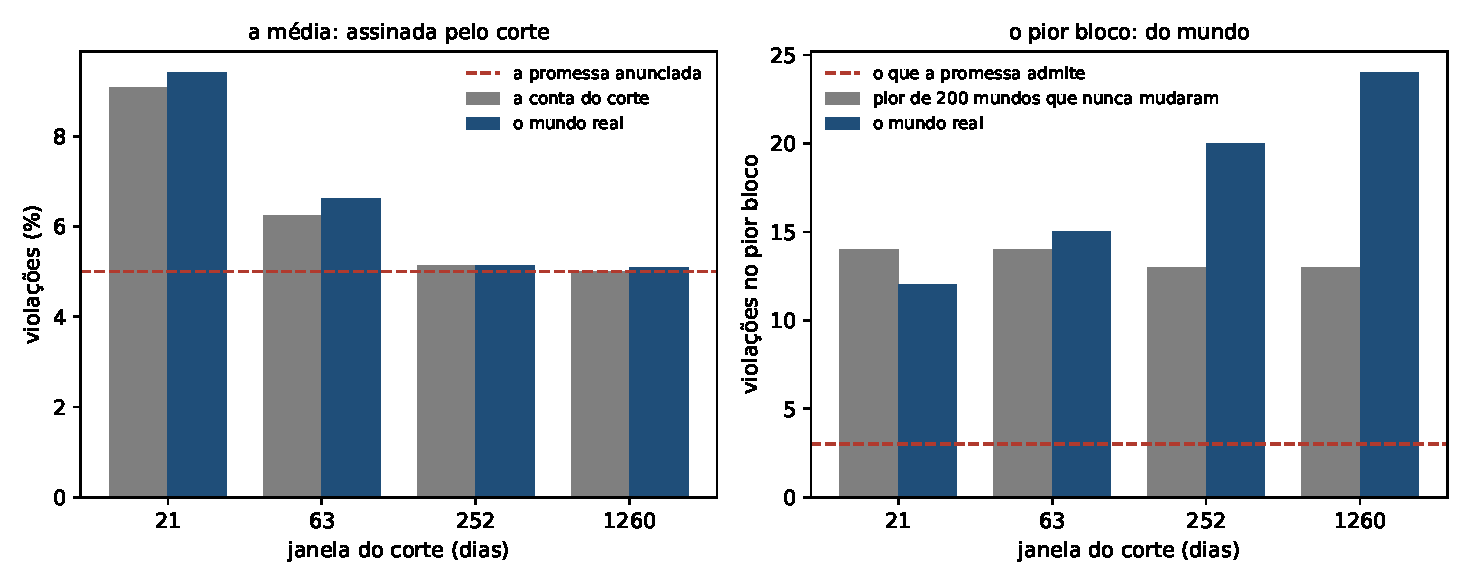
\includegraphics[width=\linewidth]{figuras/E01_promessa_2.pdf}
  \caption{As duas leituras, nas quatro janelas. À esquerda, a média: a conta do corte e o
    mundo real andam juntos. À direita, o pior bloco: o mundo real contra o pior dos
    \numNuncaMudaMundos{} mundos que nunca mudam.}
  \label{fig:duas}
\end{figure}

Encurtar o corte cobra na média; alongá-lo cobra no bloco. Não há janela em que a linha
entregue o que a promessa anunciou, e a razão disso está na \cref{prop:conta}, que não deixa o
mundo entrar na conta.

\section{Uma linha erguida no passado}

Um corte fixo supõe que o pedaço de passado que ele olha se parece com o pedaço que vem. A
série deixa de se parecer consigo mesma: passa meses colada na linha e depois rompe a linha
\numBlocoPior{} vezes em \numBlocoDias{} dias, com o pior bloco terminando em
\numBlocoPiorData.

Quando isso acontece, a linha erra por muito. Ela foi erguida com os dias de antes, e são
justamente esses dias que deixaram de valer. A \cref{tab:varredura} já mostrava o mesmo por
outro caminho, porque quanto mais longo o passado que a linha olha, mais tempo ela leva para
acompanhar o que mudou, e mais violações cabem no pedaço ruim.

Se os blocos têm data, alguma coisa no mundo se move, e a média olha para outro lugar. Resta
medir essa mudança, e os capítulos seguintes fazem isso.

\section{O que fica}

Fica o instrumento, e ele é uma linha: o $k$-ésimo pior dos últimos $n$ dias, que assina a taxa
$k/(n+1)$ antes de qualquer dado chegar. Fica também o primeiro preço medido do livro: o corte
entrega \numCorteContaPct\% onde a promessa era de \numPromessaPct\%, e essa média não distingue
o mercado de um mundo que nunca muda.

O que distingue os dois é a forma com que as violações chegam. Nos mundos que nunca mudam o pior
bloco de \numBlocoDias{} dias parou em \numNuncaMudaPiorBloco; aqui ele chegou a \numBlocoPior, em
\numBlocoPiorData.

E fica a pergunta que abre todo o resto: um corte fixo vale enquanto o passado se parecer com o que
vem, e este capítulo mostrou que ele não se parece. Medir essa mudança, e o que se pode fazer com
um alarme que chega depois dela, é o que vem.
